\documentclass{article}
\usepackage[utf8]{inputenc}
\usepackage[margin=0.75in]{geometry}
\usepackage{cite}
\usepackage{colortbl}
\usepackage{booktabs}% http://ctan.org/pkg/booktabs
\newcommand{\tabitem}{~~\llap{\textbullet}~~}
\usepackage[hidelinks]{hyperref}
\usepackage{subcaption}
\usepackage{graphicx}
\usepackage{titlesec}% http://ctan.org/pkg/titlesec
\titleformat{\section}%
    [hang]% <shape>
    {\normalfont\bfseries\Large}% <format>
    {}% <label>
    {0pt}% <sep>
    {}% <before code>
\renewcommand{\thesection}{}% Remove section references...
\renewcommand{\thesubsection}{\arabic{subsection}}%... from subsections
\usepackage{bookmark}
\usepackage{enumitem}
\usepackage{multicol}
\usepackage[figuresleft]{rotating}

\begin{document}
\begin{center}

    % MAKE SURE YOU TAKE OUT THE SQUARE BRACKETS

    \LARGE{\textbf{COMP 3004 - Deliverable \#3 \\ System Architecture and Design}}\\ 
    % \vspace{1em}
    \Large{\href{https://github.com/alextrosta/brackit}{\texttt{Brackit}} - Mobile Tournament Bracket Creation} 
    % \vspace{1em}
    % \normalsize\textbf{Jaime Herzog, Suohong Liu, Xiyi Liu, Alex Trostanovsky} \\
    % \normalsize{
    %     \href{mailto:jaime.herzog@carleton.ca}{jaime.herzog@carleton.ca},
    %     \href{mailto:suohong.liu@carleton.ca}{suohong.liu@carleton.ca},
    %     \href{mailto:xiyi.liu@carleton.ca}{xiyi.liu@carleton.ca},
    %     \href{mailto:alex.trostanovsky@carleton.ca}{alex.trostanovsky@carleton.ca}
    % }\\
    % \normalsize{
    %     101009321,
    %     101002340,
    %     101004577,
    %     100984702,
    % }
    % \vspace{1em}
    % \normalsize{Carleton University, School of Computer Science} \\
\end{center}
% \begin{normalsize}

% \end{normalsize}

\section*{Metadata}
\subsection*{Team / App Name: \href{https://github.com/alextrosta/brackit}{\texttt{Brackit}}}
% \textbf{Team Member Names:}\\ Jaime Herzog: 101009321, Suohong Liu: 101002340, Xiyi Liu: 101004577, Alex Trostanovsky: 100984702


\subsection*{Team member names}
\begin{center}
    \begin{tabular}{ |l|c| }
        \hline
        \textbf{Name}     & \textbf{Student ID} \\
        \hline
        Jaime Herzog      & 101009321           \\
        Suohong Liu       & 101002340           \\
        Xiyi Liu          & 101004577           \\
        Alex Trostanovsky & 100984702           \\
        \hline
    \end{tabular}
\end{center}
\tableofcontents
\clearpage
\section{Architecture}
% identify, describe, and justify the architecture of your project (architectural style, design patterns) \\
% Outcome is a system architecture that supports the functional goals and non-functional attributes of your project 
\subsection{Description}
In developing \texttt{Brackit}, we set out to address an urgent need by tournament attendants and organizers to visualize, manage, and interact with double elimination
brackets on their mobile devices. At a high level, we committed to developing a product that will meet the following \textbf{functional requirements}:
\begin{enumerate}
    \item{Tournament Organizers (TO's) can create, host, maintain, and visualize double elimination brackets.}
    \item{Registerd \texttt{Brackit} Users, as well as Guests, can use the application to join created tournaments.}
    \item{\texttt{Brackit} will store and maintain user profiles that will describe users' history:
    \begin{itemize}
        \item{Matches won/lost}
        \item{Tournaments entered/created}
    \end{itemize}
    }
\end{enumerate}
In terms of \textbf{non-functional requirements}, we believed \texttt{Brackit} be \textit{usable} on mobile devices. \texttt{Brackit} users should be able to:
\begin{itemize}
    \item{View and access all submodules (Brackets, Rounds, Matches) of a tournament on an Android device}
    \item{Seamlessly enter tournament competitors to brackets on an Android device}
\end{itemize}

Conceptually, \texttt{Brackit} needed to support the creation and maintenance of the following \textit{components}:
\begin{itemize}
    \item{\textit{Tournament}: The highest level abstraction utilized in Bracket creation. A tournament acts a \textit{container} for brackets.}
    \item{\textit{Bracket}: Given the number of entrants and their corresponding seeds (ranks), 
    Double elimination brackets dictate competitor matchups and the progression of competitors through the Winners and Losers brackets }
    
\end{itemize}  
\subsection{Justification}
To deve
\clearpage
\subsection{Architectural Diagrams}
\vfill
\begin{center}
    \begin{figure}[htp]
        \centering
        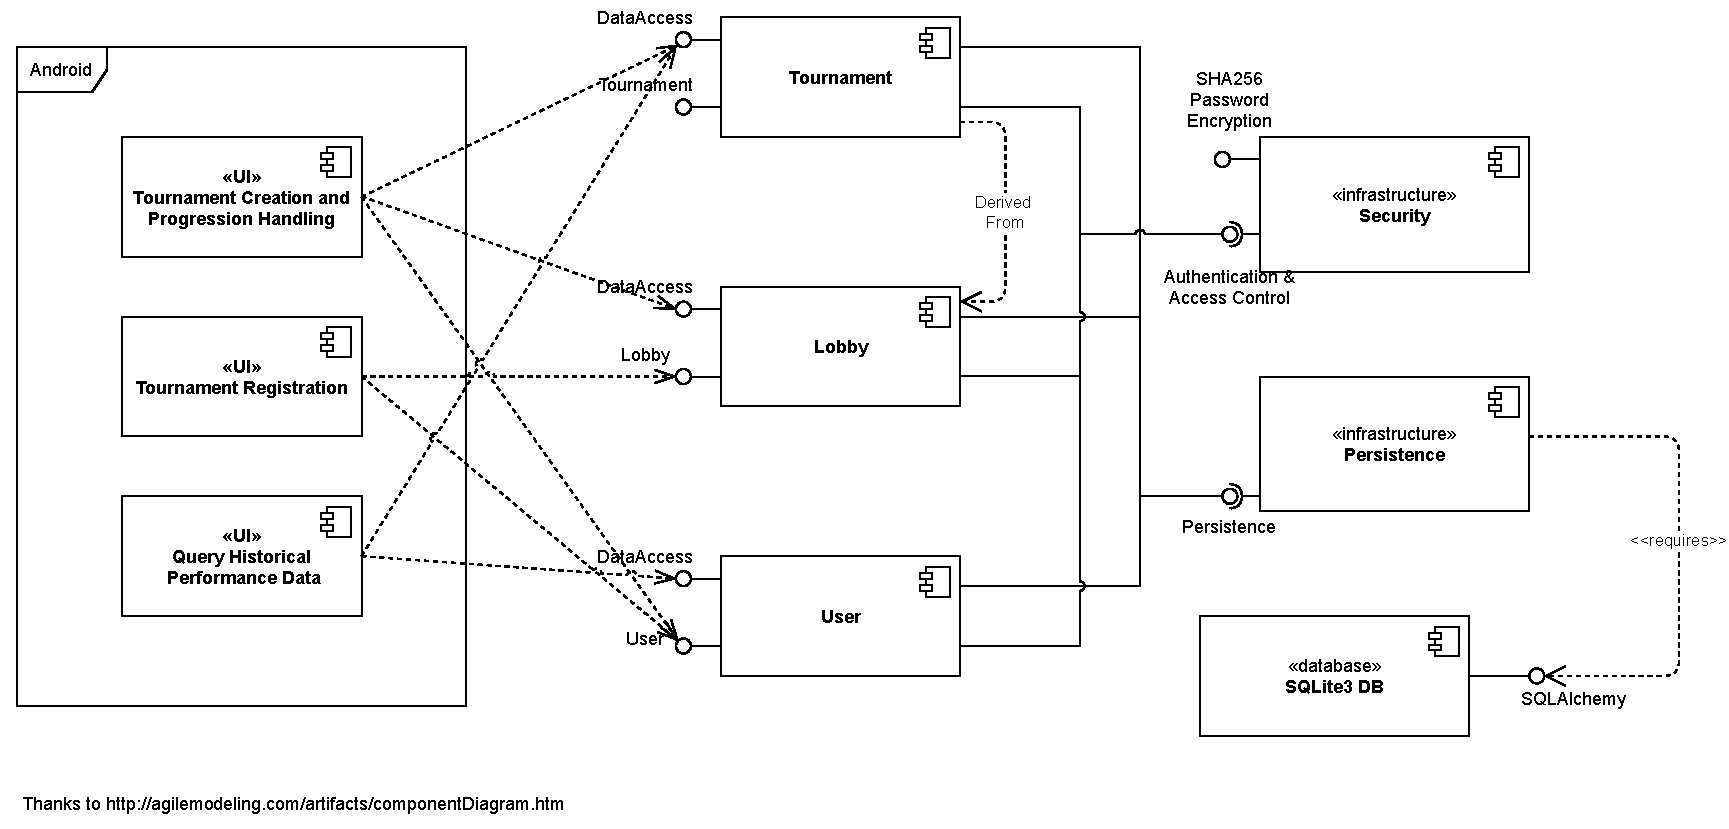
\includegraphics[width=18cm]{../diagrams/component_diag.pdf}
        \caption{\texttt{Brackit - }\href{https://sparxsystems.com/resources/tutorials/uml2/index.html}{UML 2} Architectural Component Diagram}
        \end{figure}
\end{center}
\vfill

\begin{center}
    \begin{figure}[h]
        \centering
        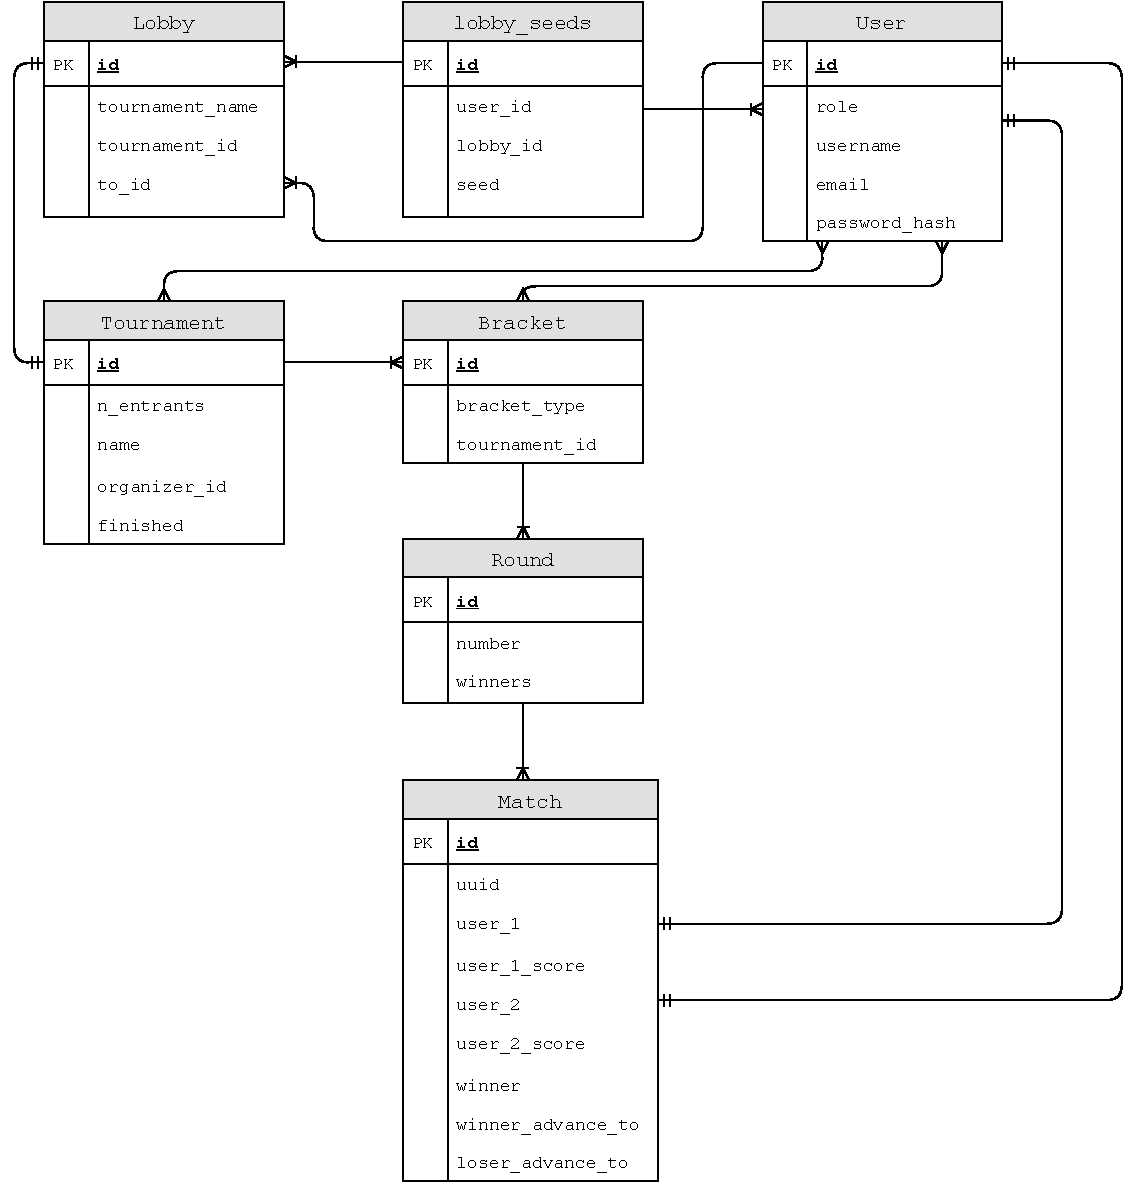
\includegraphics[width=19cm]{../diagrams/er.pdf}
        \caption{\texttt{Brackit - } Entity Relationship (ER) Diagram}
        \end{figure}
\end{center}
\clearpage
\section{Design}
\subsection{Description and Rationalization}
\begin{itemize}
    \item{Use clear description of the structure of the components and its externally visible interfaces}
    \item{Clarify the physical location of where the classes will reside (e.g., on the client, on a server),
    as well as any external API}
    \item{Include references to your system’s architecture (patterns, abstractions, data structures/
    algorithms)}
    \item{An analysis of how your design minimizes coupling and accommodates changing requirements}
\end{itemize}
\clearpage
\section{Design Diagrams}
\begin{center}
    \begin{figure}[htp]
        \centering
        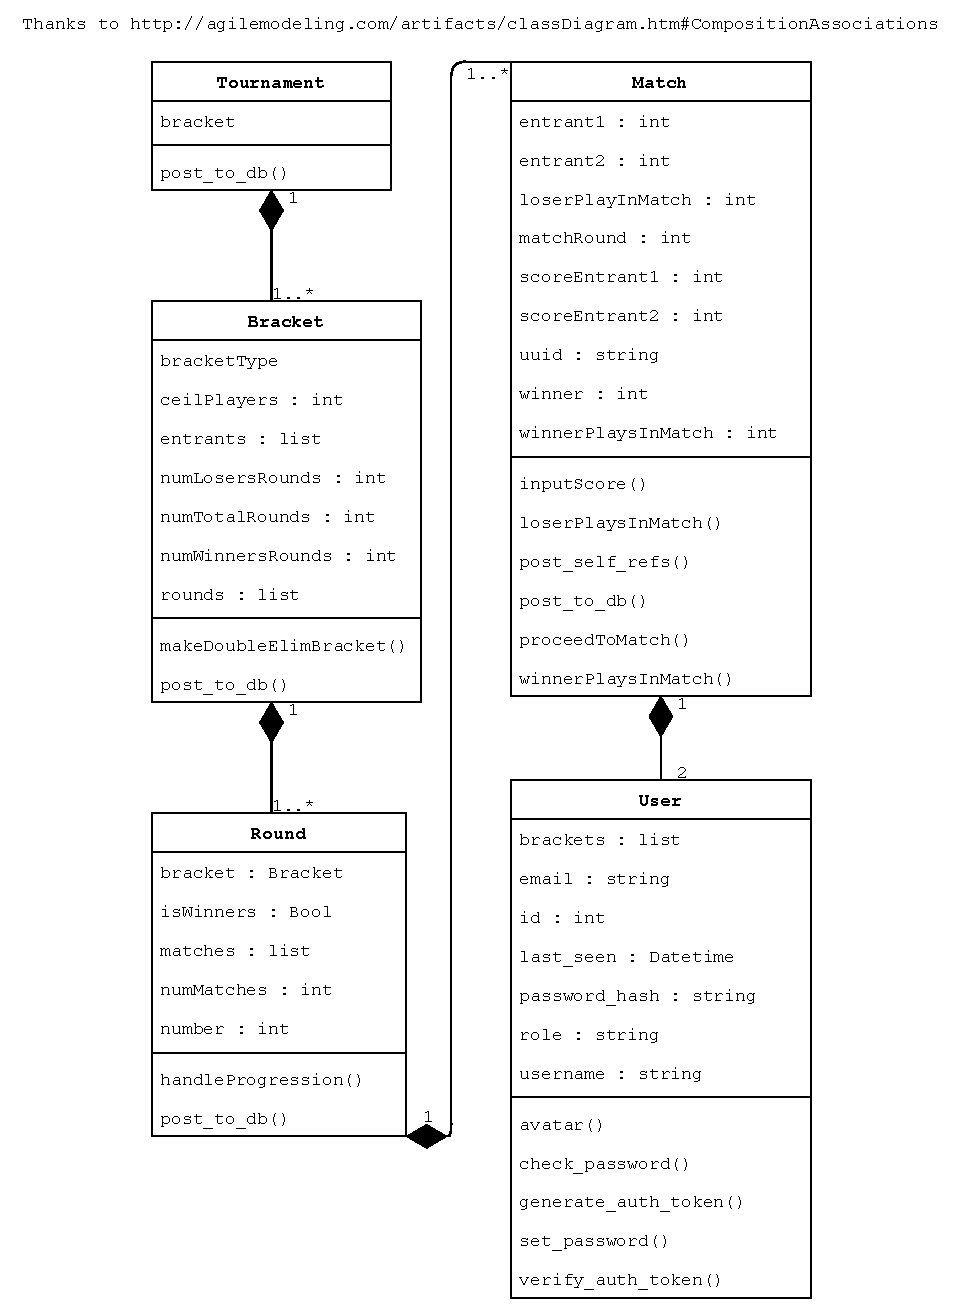
\includegraphics[width=13cm]{../diagrams/uml_class_tourn.pdf}
        \caption{\texttt{Brackit - }UML Class Diagram}
        \end{figure}
\end{center}



\clearpage
\cite{wiki:xxx}
\bibliographystyle{unsrt}
\bibliography{ref.bib}


\end{document}